%%%%%%%%%%%%%%%%%%%% author.tex %%%%%%%%%%%%%%%%%%%%%%%%%%%%%%%%%%%
%
% sample root file for your "contribution" to a contributed volume
%
% Use this file as a template for your own input.
%
%%%%%%%%%%%%%%%% Springer %%%%%%%%%%%%%%%%%%%%%%%%%%%%%%%%%%


% RECOMMENDED %%%%%%%%%%%%%%%%%%%%%%%%%%%%%%%%%%%%%%%%%%%%%%%%%%%
\documentclass[graybox]{svmult}

% choose options for [] as required from the list
% in the Reference Guide

\usepackage{mathptmx}       % selects Times Roman as basic font
\usepackage{helvet}         % selects Helvetica as sans-serif font
\usepackage{courier}        % selects Courier as typewriter font
\usepackage{type1cm}        % activate if the above 3 fonts are
                            % not available on your system
%
\usepackage{makeidx}         % allows index generation
\usepackage{graphicx}        % standard LaTeX graphics tool
                             % when including figure files
\usepackage{subfigure}
\usepackage{epstopdf}

\usepackage{multicol}        % used for the two-column index
\usepackage[bottom]{footmisc}% places footnotes at page bottom
\usepackage{amsmath}
\usepackage{amssymb}
\usepackage{mathtools}
%\usepackage[linesnumbered, ruled, vlined]{algorithm2e}
%\usepackage{algorithm}% http://ctan.org/pkg/algorithms
%\usepackage{algorithmicx} 
%\usepackage{algpseudocode}% http://ctan.org/pkg/algorithmicx
%\renewcommand{\algorithmicrequire}{\textbf{Input:}}
%\renewcommand{\algorithmicensure}{\textbf{Output:}}
\usepackage{enumerate}
\usepackage{multirow}
\usepackage{cleveref}

\usepackage[hang, small,labelfont=bf,up,textfont=it,up]{caption} % Custom captions under/above floats in tables or figures
\usepackage{booktabs} % Horizontal rules in tables
\usepackage{float} % Required for tables and figures in the multi-column environment - they need to be placed in specific locations with the [H] (e.g. \begin{table}[H])
%\usepackage{hyperref} % For hyperlinks in the PDF

% see the list of further useful packages
% in the Reference Guide

\makeindex             % used for the subject index
                       % please use the style svind.ist with
                       % your makeindex program

%%%%%%%%%%%%%%%%%%%%%%%%%%%%%%%%%%%%%%%%%%%%%%%%%%%%%%%%%%%%%%%%%%%%%%%%%%%%%%%%%%%%%%%%%

\begin{document}

\title*{Model Order Redcution of Fluid Flow While Preserving Quadratic Invariants}
% Use \titlerunning{Short Title} for an abbreviated version of
% your contribution title if the original one is too long
\author{Bababk Maboudi Afkham, Nicol\`o Ripamonti, Qian Wang, Jan S. Hesthaven and Karen E. Willcox}
% Use \authorrunning{Short Title} for an abbreviated version of
% your contribution title if the original one is too long
\institute{Name of First Author \at Name, Address of Institute, \email{name@email.address}
\and Name of Second Author \at Name, Address of Institute \email{name@email.address}}
%
% Use the package "url.sty" to avoid
% problems with special characters
% used in your e-mail or web address
%
\maketitle

%\abstract*{Each chapter should be preceded by an abstract (10--15 lines long) that summarizes the content. The abstract will appear \textit{online} at \url{www.SpringerLink.com} and be available with unrestricted access. This allows unregistered users to read the abstract as a teaser for the complete chapter. As a general rule the abstracts will not appear in the printed version of your book unless it is the style of your particular book or that of the series to which your book belongs.
%Please use the 'starred' version of the new Springer \texttt{abstract} command for typesetting the text of the online abstracts (cf. source file of this chapter template \texttt{abstract}) and include them with the source files of your manuscript. Use the plain \texttt{abstract} command if the abstract is also to appear in the printed version of the book.}

\abstract{In the context of model order reduction, conservation of stability in the reduced order systems of partial differential equation, especially with a strong advection term, remains a challenge. Recently preserving structures, invariants and conservation laws, in order to help with stability, and ensure robustness in long-time integrations, has been an area of active research. Energy conservation is a fundamental feature of fluid flows which is often violated in the course of model reduction. In this paper we discuss a model reduction routine, that exploits skew-symmetry of conservative and centered discretization schemes, to recover conservation of energy at the level of reduced system. This results in an, overall, correct evolution of the fluid and ensures robustness of the reduced system. We evaluate the performance of the proposed method through numerical simulation of various fluid flows, and also in a numerical simulation of continuous variable resonance combustor model.}


% sections are added here

\section{Introduction}
\label{sec:intro}

Reduced order models have emerged as a powerful approach to cope with increasingly complex new applications in engineering and science. These methods substantially reduce the dimensionality of the problem by constructing a reduced configuration space. Exploration of the reduced space is then possible with significant acceleration \cite{hesthaven2015certified,Haasdonk2017}.

Over the past decade, reduced basis (RB) methods have demonstrated great success in lowering of the computational costs of solving elliptic and parabolic differential equations \cite{ito1998reduced,ito2001reduced}. However, model order reduction (MOR) of hyperbolic problems remains a challenge. Such problems often arise from a set of conservation laws and invariants. These intrinsic structures are lost during MOR which results in a qualitatively wrong, and sometimes unstable reduced system \cite{Amsallem:2014ef}.

%To have a sense of this error, error estimation is important from applications point of view \cite{HaasdonkOhlberger11,RuinerEtAl12,BhattEtAl18}. But it can difficult and expensive to compute useful error bounds. When one is interested in a cheap surrogate for the error incurred or when the conserved quantity is an output of the system, it becomes imperative to preserve this structure through model order reduction.

Recently, the construction of RB methods that conserve intrinsic structures has attracted attention \cite{doi:10.1137/17M1111991,1705.00498,kalashnikova2014stabilization,farhat2015structure,doi:10.1137/110836742,doi:10.1137/140959602,beattie2011structure,doi:10.1137/140978922}. Structure preservation in MOR not only constructs a physically meaningful reduced system, but can also enhance the robustness and stability of the reduced system. In system theory, conservation of passivity can be found in the work of \cite{polyuga2010structure,gugercin2012structure}. Energy preserving and inf-sup stable methods for finite element methods (FEM) are developed in \cite{farhat2015structure,ballarin2015supremizer}. Also, a conservative MOR technique for finite-volume methods is proposed in \cite{1711.11550}.

Moreover, the simulation of reduced models incurs solution errors and the estimation of this error is essential in applications of MOR \cite{HaasdonkOhlberger11,RuinerEtAl12,BhattEtAl18}. Finding tight error bounds for a general reduced system has shown to be computationally expensive and often impractical. Therefore, when one is interested in a cheap surrogate for the error or when the conserved quantity is an output of the system, it becomes imperative to preserve system structures in the reduced model.

In the context of Lagrangian and Hamiltonian systems, recent works provide a promising approach to the construction of robust and stable reduced systems. Carlberg, Tuminaro, and Boggs \cite{Carlberg:2014ky} suggest that a reduced order model of a Lagrangian system be identified by an approximate Lagrangian on a reduced order configuration space. This allows the reduced system to inherit the geometric structure of the original system. A similar approach has been adopted in the work of Peng and Mohseni \cite{doi:10.1137/140978922} and in the work of Maboudi Afkham and Hesthaven \cite{doi:10.1137/17M1111991} for Hamiltonian systems. They construct a low-order symplectic linear vector space, i.e. a vector space equipped with a symplectic 2-form, as the reduced space. Once the symplectic reduced space is generated, a symplectic projection result in a physically meaningful reduced system. A proper time-stepping scheme then preserves the Hamiltonian structure of the reduced system. It is shown in \cite{doi:10.1137/17M1111991,doi:10.1137/140978922} that this approach preserves the overall dynamics of the original system and enhances the stability of the reduced system. Despite the success of these method in MOR of Hamiltonian systems, these techniques are only compatible with the Euclidean inner product. Therefore, the computational structures that arise from a natural inner product of a problem will be lost during MOR.

Weak formulations and inner-products, defined on a Hilbert space, are at the core of the error analysis of many numerical methods for solving partial differential equations. Therefore, it is natural to seek MOR methods that consider such features. At the discrete level, these features often require a Euclidean vector space to be equipped with a generalized inner product, associated with a weight matrix $X$. Many works enabled conventional MOR techniques compatible with such inner products \cite{sen2006natural}. However, a MOR method that simultaneously preserves the symplectic symmetry of Hamiltonian systems remains unknown. 

In this paper, we seek to combine a classical MOR method with respect to a weight matrix with the symplectic MOR. The reduced system constructed by the new method is a generalized Hamiltonian system and the low order configuration space associated with this system is a symplectic linear vector space with a non-standard symplectic 2-form. It is demonstrated that the new method can be viewed as the natural extension to \cite{doi:10.1137/17M1111991}, and therefore retains the structure preserving features, e.g. symplecticity and stability. We also present a greedy approach for the construction of a generalized symplectic basis for the reduced system. Structured matrices are in general not norm bounded \cite{Karow:2006cf}. However, we show that the condition number of the basis generated by the greedy method is bounded by the condition number of the weight matrix $X$. Finally, to accelerate the evaluation of nonlinear terms in the reduced system, we present a variation of the discrete empirical interpolation method (DEIM) that preserves the symplectic structure of the reduced system.

What remains of this paper is organized as follows. In \cref{sec:hamil} we cover the required background on the Hamiltonian and the generalized Hamiltonian systems. \Cref{sec:mor} summarizes classic MOR routine with respect to a weighted norm and the symplectic MOR method with respect to the standard Euclidean inner product. We introduce the symplectic MOR method with respect to a weighted inner product in \cref{sec:normmor}. \Cref{sec:res} illustrates the performance of the new method through a vibrating beam and the sine-Gordon equation. We offer a few conclusive remarks in \cref{sec:conc}.

\section{Model Order Reduction} \label{chap:MoOr:1}
Consider a parameterized, finite dimensional dynamical system described by a set of first order ordinary differential equations
\begin{equation} \label{eq:MoOr:1}
\left\{
\begin{split}
& \frac{d}{dt} \mathbf{x}(t,\omega) = \mathbf f (t,\mathbf x,\omega), \\
& \mathbf x(0,\omega) = \mathbf x_0(\omega).
\end{split}
\right.
\end{equation}
Here $\mathbf x \in \mathbb R^n$ is the state vector, $\omega \in \Gamma$ is a vector containing all the parameters of the system {\edit belonging} to a compact set $\Gamma$ ($\subset \mathbb R^d$) and $\mathbf f : \mathbb R \times \mathbb R^n \times \Gamma \to \mathbb R^n$ is a general {\edit vector valued} function of the state variables and parameters.

We define the solution manifold as the set of all solutions to (\ref{eq:MoOr:1}) under variation of {\edit the parameters in $\Gamma$}
\begin{equation} \label{eq:MoOr:2}
	\edit \mathcal M = \{ \mathbf x(t,\omega) | \omega \in \Gamma,\ t\geq 0 \} \subset \mathbb R^n.
\end{equation}
Note that the exact solution and solution manifold is {\edit often not} available; we assume that we have a numerical integrator that can approximate the solution to (\ref{eq:MoOr:1}) for any realization of $\omega$ {\edit with a given accuracy}. By abuse of notation, we refer to $\mathbf x$ and $\mathcal M$ as the exact solution and the exact solution manifold, respectively, rather than the discrete solution and discrete solution manifold. 

Model order reduction is based on the assumption that $\mathcal M$ is of low dimension \cite{Anonymous:2016wl,Antoulas:2005:ALD:1088857} and that the span of appropriately chosen basis vectors $\{v_i\}_{i=1}^k$ covers most of the solution manifold {\edit to within} a small error. The set $\{v_i\}_{i=1}^k$ is denoted as the \emph{reduced basis} and its span as the \emph{reduced space}. Assuming that a $k$-dimensional $(k\ll n)$ reduced basis is given, the approximated solution can be represented as
\begin{equation} \label{eq:MoOr:3}
	\mathbf x \approx V \mathbf y,
\end{equation}
where $V$ is a matrix containing the reduced basis vectors as its columns and $\mathbf y$ {\edit contains} the coordinates of the approximation in this basis. By substituting (\ref{eq:MoOr:3}) into (\ref{eq:MoOr:1}) we obtain the overdetermined system
\begin{equation} \label{eq:MoOr:4}
	V \frac{d}{dt} \mathbf y = \mathbf f (t , V \mathbf y , \omega) + \mathbf r(t,\omega).
\end{equation}
Here we added the residual $\mathbf r$ to emphasize that (\ref{eq:MoOr:4}) is an approximation of (\ref{eq:MoOr:1}). Taking the Petrov-Galerkin projection \cite{Antoulas:2005:ALD:1088857} we construct a basis $W$ of size $n-k$ that is orthogonal to the residual $\mathbf r$ and {\edit requires that} $W^T V$ is invertible. This yields
\begin{equation} \label{eq:MoOr:5}
	\frac{d}{dt} \mathbf y = (W^TV)^{-1} \mathbf f(t,V\mathbf y,\omega).
\end{equation}
Equation (\ref{eq:MoOr:5}) consists of $k$ equations and is called the reduced system. Solving the reduced system instead of the original system can reduce the computational costs {\edit provided} $k$ is significantly smaller than $n$. For nonlinear systems, the evaluation of $\mathbf f$ may still have computational complexity that depends on $n$. We return to this question in detail in Section \ref{chap:MoOr.DEIM:1}.

\subsection{Proper Orthogonal Decomposition} \label{chap:MoOr.PrOr:1}
Let $\mathbf x (t_i,\omega_j)$ with $i=1,\dots,m$ and $j=1,\dots,n$ be a finite number of samples, referred to as \emph{snapshots}, from the solution manifold (\ref{eq:MoOr:2}). If we {\edit assume} that a reduced basis $V$ is provided, the projection operator from $\mathbb R^n$ onto the reduced space can be constructed as $VV^T$. The proper orthogonal decomposition (POD) requires the total error of projecting all the snapshots onto the reduced space to be {\edit minimized}. The POD basis of size $k$ is thus the solution to the optimization problem
\begin{equation} \label{eq:MoOr:6}
\begin{aligned}
& \underset{V\in \mathbb R^{n\times k}}{\text{minimize}}
& & \| S - VV^TS\|_F \\
& \text{subject to}
& & V^TV = I_k
\end{aligned}
\end{equation}
Here $S$ is the snapshot matrix, containing snapshots $\mathbf x(t_i,\omega_j)$ in its columns, $\|\cdot \|_F$ is the Frobenius norm and $I_k$ is the identity matrix of size $k$. According to {\blue the} {\edit Schmidt-Mirsky-Eckart-Young theorem \cite{Markovsky:2011:LRA:2103589}}, the solution to (\ref{eq:MoOr:6}) is equivalent to the truncated singular value decomposition (SVD) of the snapshot matrix $S$ given by
\begin{equation} \label{eq:MoOr:7}
	V = \sigma_1 u_1 v^T_1 + \cdots + \sigma_k u_k v^T_k.
\end{equation}
Here $\sigma_i, u_i$ and $v_i$ are the singular values, the left singular vectors, and the right singular vectors of $S$, respectively {\edit \cite{Markovsky:2011:LRA:2103589} }.


\subsection{Discrete Empirical Interpolation Method (DEIM)} \label{chap:MoOr.DEIM:1} \nocite{Chaturantabut:2010cz}
In this section we {\edit discuss the efficiency} of evaluating nonlinearities {\edit in the context of} projection based reduced models. Suppose that the right hand side in (\ref{eq:MoOr:1}) is of the form $\mathbf f(t,\mathbf x , \omega) = L\mathbf x + \mathbf g(t,\mathbf x ,\omega)$, where $L\in \mathbb R^{n\times n}$ reflects the linear part, and $\mathbf g$ is a nonlinear function. Now {\edit assume that} a $k$-dimensional reduced basis $V$ is provided. The reduced system takes the form
\begin{equation} \label{eq:MoOr:8}
	\frac{d}{dt} \mathbf y = \underbrace{(W^TV)^{-1} L V}_{\tilde L} \mathbf{y} + \underbrace{(W^TV)^{-1} \mathbf g(t,V\mathbf y,\omega)}_{\tilde N (\mathbf y)}.
\end{equation}
Here, $\tilde L$ is a $k\times k$ matrix which can be computed before time integration of the reduced system. However, {\edit the} evaluation of $\tilde N (\mathbf y)$ has a complexity that depends on $n$, the size of the original system. Suppose that the evaluation of $\mathbf g$ with $n$ components has the complexity $\alpha(n)$, for some function $\alpha$. Then the complexity of evaluating $\tilde N(\mathbf y)$ is $\mathcal{O}(\alpha(n) + 4nk)$ which consists of 2 matrix-vector operations and the {\edit evaluation of the nonlinear function, i.e. the evaluation of the nonlinear terms can be as expensive as solving the original system.}

{\edit To overcome this bottleneck we take an approach similar to that of Section \ref{chap:MoOr.PrOr:1} \cite{Chaturantabut:2010cz,Barrault:2004kz}}. Assume that the manifold $\mathcal M_{\mathbf g} = \{ \mathbf g(t,\mathbf x , \omega)| t\in \mathbb R, \mathbf x \in \mathbb R , \omega \in \Gamma\}$ is of a low dimension and that $\mathbf g$ can be approximated by a linear subspace of dimension $m\ll n$, spanned by the basis $\{ u_1 , \dots , u_m \}$, i.e.
\begin{equation} \label{eq:MoOr:10}
	\mathbf g(t,\mathbf x,\omega) \approx U \mathbf c(t,\mathbf x,\omega).
\end{equation}
Here $U$ contains basis vectors $u_i$ and $\mathbf c$ is the vector of coefficients. Now suppose $p_1,\dots,p_m$ are $m$ indices from $\{1,\dots,n\}$ and define an $n\times m$ matrix
\begin{equation} \label{eq:MoOr:11}
	P = [e_{p_1},\dots,e_{p_m}],
\end{equation}
where $e_{p_i}$ is the $p_i$-th column of the identity matrix $I_n$. Multiplying $P$ with $\mathbf g$ selects components $p_1,\dots,p_m$ of $\mathbf g$. If we assume that $P^TU$ is non-singular, the coefficient vector $\mathbf c$ can be uniquely determined from
\begin{equation} \label{eq:MoOr:12}
	P^T \mathbf g = (P^TU)\mathbf c.
\end{equation}
Finally the approximation of $\mathbf g$ is determined by
\begin{equation} \label{eq:MoOr:13}
	\mathbf g(t,\mathbf x,\omega) \approx U \mathbf c(t,\mathbf x,\omega) = U (P^TU)^{-1} P^T \mathbf g(t,\mathbf x,\omega),
\end{equation}
which is referred to as the \emph{Discrete Empirical Interpolation} (DEIM) approximation \cite{Chaturantabut:2010cz}. Applying DEIM to the reduced system (\ref{eq:MoOr:5}) yields
\begin{equation} \label{eq:MoOr:14}
	\frac{d}{dt} \mathbf y = \tilde L \mathbf y + (WV)^{-1} U(P^TU)^{-1}P^T \mathbf g(t,V\mathbf y , \omega).
\end{equation}
Note that the matrix $(WV)^{-1} U(P^TU)^{-1}$ can be computed offline and since $\mathbf g$ is evaluated only at $m$ of its components, the evaluation of the nonlinear term in (\ref{eq:MoOr:14}) does not depend on $n$.

{\edit To obtain the projection basis $U$, the POD can be applied to the ensemble of samples of the nonlinear term $\mathbf g(t_i,\mathbf x, \omega_j)$ with $i=1,\dots,m$ and $j=1,\dots,n$}. There is no additional cost {\edit associated with} computing the nonlinear snapshots, since they are generated when computing the trajectory snapshot matrix $S$. The interpolating indices $p_1,\dots,p_m$ can be constructed as follows. Given the projection basis $U = \{u_1,\dots,u_m\}$, the first interpolation index $p_1$ is chosen according to the component of $u_1$ with the largest magnitude. The rest of the interpolation indices, $p_2,\dots,p_m$ correspond to the component of the largest magnitude of the residual vector $\mathbf r = u_l - U \mathbf c$. It is shown in \cite{Chaturantabut:2010cz} that if the residual vector is a nonzero vector in each iteration then $P^TU$ is non-singular and (\ref{eq:MoOr:13}) is well defined. 

\begin{algorithm} 
\caption{Discrete Empirical Interpolation Method} \label{alg:MoOr:1}
{\bf Input:}  Basis vectors $\{u_1,\dots , u_m\}\subset \mathbb R^n$
\begin{enumerate}
\item pick $p_1$ to be the index of the largest component of $u_1$.
\item $U \leftarrow [u_1]$
\item $P \leftarrow [p_1]$
\item \textbf{for} $i\leftarrow 2$ \textbf{to} $m$
\item \hspace{0.5cm} solve $(P^TU)\mathbf c = P^T u_i$ for $\mathbf c$
\item \hspace{0.5cm} $\mathbf r \leftarrow u_i - U\mathbf c$
\item \hspace{0.5cm} pick $p_i$ to be the index of the largest component of $\mathbf r$
\item \hspace{0.5cm} $U \leftarrow [u_1,\dots,u_i]$
\item \hspace{0.5cm} $P \leftarrow [p_1,\dots,p_i]$
\item \textbf{end for}
\end{enumerate}
\vspace{0.5cm}
{\bf Output:} Interpolating indices $\{p_1,\dots,p_m\}$
\end{algorithm}


{\edit The numerical solution of (\ref{eq:MoOr:8}) may involve the computation of the Jacobian of the nonlinear function $\mathbf g(t,\mathbf x, \omega)$ with respect to the reduced state variable $\mathbf y$}
\begin{equation} \label{eq:MoOr:9}
	\edit \mathbf J_{\mathbf y}(\mathbf g) = (WV)^{-1} \mathbf J_{\mathbf x}(\mathbf g) V,
\end{equation}
{\edit where $\mathbf J_\alpha(\mathbf g)$ is the Jacobian matrix of $\mathbf g$ with respect to the variable $\alpha$.} The complexity of (\ref{eq:MoOr:9}) is $\mathcal{O}(\alpha(n) +2n^2k+2nk^2+2nk)$, comprising several matrix-vector multiplications and an evaluation of the Jacobian which depends on the size of the original system. Approximating the Jacobian in (\ref{eq:MoOr:9}) is usually both problem and discretization dependent. Often the nonlinear function $\mathbf g$ is evaluated component-wise i.e.
\begin{equation} \label{eq:MoOr:15}
	\mathbf g(\mathbf x) =
	\begin{pmatrix}
		g_1(x_1,\dots,x_n) \\
		g_2(x_1,\dots,x_n) \\
		\vdots \\
		g_n(x_1,\dots,x_n)
	\end{pmatrix}
	=
	\begin{pmatrix}
		g_1(x_1) \\
		g_2(x_2) \\
		\vdots \\
		g_n(x_n)
	\end{pmatrix}.
\end{equation}
In such cases the interpolating index matrix $P$ and the nonlinear function $\mathbf g$ commute, i.e.,
\begin{equation} \label{eq:MoOr:16}
	\tilde N(\mathbf y) \approx (WV)^{-1} U(P^TU)^{-1}P^T \mathbf g(V\mathbf y) = (WV)^{-1} U(P^TU)^{-1}\mathbf g(P^TV\mathbf y)
\end{equation}
If we now take the Jacobian of the approximate function we recover
\begin{equation}
	\edit \mathbf J_{\mathbf y}(\mathbf g) = \underbrace{ (WV)^{-1} U(P^TU)^{-1} }_{k\times m} \underbrace{ \mathbf J_{\mathbf x}(\mathbf g(P^T V \mathbf y) ) }_{m\times m} \underbrace{P^T V}_{m\times k}.
\end{equation}
The matrix $(WV)^{-1} U(P^TU)^{-1}$ can be computed offline and the Jacobian is evaluated only for $m\times m$ components. Hence the overall complexity of computing the Jacobian is now independent of $n$. {\edit We refer the reader to \cite{Barrault:2004kz,Chaturantabut:2010cz} for more detail.}

\section{Skew Symmetric and Centered Schemes for Fluid Flows} \label{sec:skew}

\subsection{Conservation Laws} \label{sec:skew.1}
Transport of conserved quantities, in the context of fluid flows, can be formulated as
\begin{equation} \label{eq:3.1}
	\frac{\partial }{\partial t} \rho \varphi + \nabla \cdot ( \rho u \varphi  ) = \nabla \cdot F_{\varphi}\quad \text{defined in} \quad \Omega \subset \mathbb R^{d}.
\end{equation}
Here, $d = 1,2$ or $3$, $\rho:\Omega\to \mathbb R$ is the density, $u\in \Omega \to \mathbb R^{d}$ is the velocity vector field, $\varphi$ is a measured scalar quantity of the flow, and $F_{\varphi}$ is the flux function associated to $\varphi$. Integration of \eqref{eq:3.1} over $ \Omega$ yields
\begin{equation} \label{eq:3.2}
	\frac{d}{dt} \int_{\Omega} \rho \varphi \ dx = \int_{\partial \Omega} (F_{\varphi} - \rho u \varphi) \cdot \hat n\ ds,
\end{equation}
where $\partial \Omega$ is the boundary of $\Omega$, and $\hat n$ is the unit outward normal vector to $\partial \Omega$. When the right hand side of \eqref{eq:3.2} vanishes, e.g. in case where $\Omega$ is periodic and $\varphi$ is flux-free, the quantity $(\rho \varphi)$ is conserved. Therefore, the form \eqref{eq:3.1} is referred to the \emph{conservative form} and the convective term in \eqref{eq:3.1} is referred to as the \emph{divergence form}. However, using the \emph{continuity equation}
\begin{equation} \label{eq:3.3}
	\frac{\partial }{\partial t} \rho + \nabla \cdot (\rho u) = 0,
\end{equation}
we can rewrite \eqref{eq:3.1} as
\begin{equation} \label{eq:3.4}
	\rho \frac{\partial }{\partial t} \varphi + (\rho u)\cdot \nabla \varphi = \nabla \cdot F_{\varphi}.
\end{equation}
The convective term in this formulation is referred to as the \emph{advective form}. The \emph{skew-symmetric} form for the convective term is obtained by the arithmetic average of the divergent and the advective form:
\begin{equation} \label{eq:3.5}
	\frac{1}{2} \left( \rho \frac{\partial }{\partial t} \varphi + \frac{\partial }{\partial t} (\rho \varphi) \right) + \frac 1 2 \left( (\rho u)\cdot \nabla \varphi + \nabla \cdot (\rho u \varphi) \right) = \nabla \cdot F_{\varphi}.
\end{equation}
Multiplying \eqref{eq:3.5} with $\varphi$ yields
\begin{equation}
	\frac{\partial }{\partial t} \rho \varphi^2 + \nabla \cdot ( \rho u \varphi^2  ) = \varphi \nabla \cdot F_{\varphi}.
\end{equation}
Therefore, $\varphi^2$ is a conserved quantity for a flux-free $\varphi$. Since the divergence, the advective and the skew-symmetric forms are identical at the continuous level, then $\varphi^2$ is a conserved quantity for all forms. However, equivalence of these forms is not preserved through a general discretization scheme and, therefore, we do not expect $\varphi^2$ to be a conserved quantity in discrete level. Assuming proper boundary conditions, the operator 
\begin{equation}
	S_{\rho u}(\cdot) = \frac 1 2 ( [ \nabla \cdot \rho u ] + (\rho u)\cdot \nabla )(\cdot),
\end{equation}
is a skew-adjoint operator with respect to the $L^2$ inner-product. Here, $[\cdot]$ indicates that the inside of brackets act as a differential operator. This skew-adjoint property is used in later sections to show the conservation of some quadratic quantities in \eqref{eq:3.1}. Similarly, we can define the skew-adjoint operator in time variable as
\begin{equation}
	S_{\rho,\partial_t} = \frac{1}{2} \left( \rho \frac{\partial}{\partial t} + [ \frac{\partial}{\partial t} \rho] \right).
\end{equation}
Here, the subscript $\partial t$ is to emphasize that $S_{\rho,\partial_t}$ is a differential operator with respect to $t$. Note that numerical time integration of \eqref{eq:3.5} can be challenging since the time differentiation of different variable is present. However, following derivations in \cite{morinishi2010skew}, one can rewrite \eqref{eq:3.5} as
\begin{equation} \label{eq:3.6}
	\sqrt{\rho } \frac{\partial }{\partial t} (\sqrt \rho \varphi ) + S_{\rho u}(\varphi) = \nabla \cdot F_{\varphi}.
\end{equation}
Time integration of this form is presented in the works of \cite{?}. Note that one can also generate a quasi-skew-symmetric form \cite{blaisdell1991numerical,morinishi2003dns} of \eqref{eq:3.1} as
\begin{equation} \label{eq:3.7}
	\frac{\partial }{\partial t} (\rho \varphi) + S_{\rho u}(\varphi) = \nabla \cdot F_{\varphi}.
\end{equation}
Even though this is not a fully skew-symmetric form (skew-symmetric only in space), the numerical stabilities of this form is significantly better than the divergence and advective form \cite{morinishi2010skew,blaisdell1991numerical,morinishi2003dns}. Note that the quasi-skew-symmetric form is identical to the skew-symmetric form in the incompressible limit.

\subsection{Incompressible Fluid} \label{sec:skew.2}
Consider the governing equations of an incompressible fluid with skew-symmetric convective term:
\begin{equation} \label{eq:3.8}
	\left\{
	\begin{aligned}
	&\nabla \cdot u = 0, \\
	&\frac{\partial}{\partial t} u + S_{u}(u) + \nabla p = \nabla \cdot \tau,
	\end{aligned}
	\right.
\end{equation}
defined on $\Omega$. Here, $p: \Omega \to \mathbb R^+$ is the pressure, $\tau: \Omega \to \mathbb R^{d\times d}$ is the viscous stress tensor, and $S_u = \frac 1 2 ([ \nabla \cdot u] + u\cdot \nabla)$. It is straight forward to check
\begin{equation} \label{eq:3.9}
	\frac{d}{dt} K + \nabla \cdot (Ku) + \nabla \cdot (pu)= \nabla \cdot (\tau u) - (\tau \nabla)\cdot u,
\end{equation}
where $K = \frac 1 2 \sum_{i=1}^d u_i^2 $ is the kinetic energy. Here we used 
\begin{equation} \label{eq:3.10}
	\begin{aligned}
	u\cdot \nabla p &= \nabla \cdot (up) - p\nabla \cdot u, \\
	u \cdot (\nabla \cdot \tau) &= \nabla \cdot (\tau u) - (\tau \nabla)\cdot u,
	\end{aligned} 
\end{equation}
and
\begin{equation} \label{eq:3.11}
	u\cdot S_{u}(u) = \nabla \cdot(Ku).
\end{equation}
The only non-conservative term in \eqref{eq:3.9} is $-(\tau \nabla)\cdot u$, which corresponds to dissipation of kinetic energy. Therefore, in the absence of the viscous terms, $K$ is a conserved quantity of the system, and $\frac d {dt} \int_{\Omega} K \ dx <0$ when $\tau\neq 0$. Note that as long as $\nabla \cdot u = 0$, as discussed in \Cref{sec:skew.1}, the divergence, the convective, and the skew-symmetric forms are identical for the incompressible fluid equation. Thus, kinetic energy is conserved for all forms. However, for a general discretization scheme, these forms are not identical, and often the conservation of kinetic energy, in the discrete sense, is violated.

The skew-symmetric discretization of \eqref{eq:3.8} is a centered scheme that exploits the skew-adjoint property of $S_u$, and ensures conservation of kinetic energy at the discrete level. We uniformly discretize $\Omega$ into $N$ points and denote by $\mathbf u \in \mathbb R^{N\times d}$, $\mathbf p \in \mathbb R^N$, and $T \in R^{N\times d\times d} $ the discrete representation of $u$, $p$, and $\tau$, respectively. Let $D_j$ be the centered finite difference matrix operator for $\partial / \partial x_j$, for $j = 1,\dots,d$. The momentum equation in \eqref{eq:3.8} is then discretized as
\begin{equation} \label{eq:3.13}
	\frac{d}{dt}{\mathbf u}_i + S_{\mathbf u} \mathbf u_i + D_i \mathbf p = \sum_{j=1}^d D_j T_{ij}, \quad i=1,\dots,d.
\end{equation}
where $S_{\mathbf u}$ is the discretization of $S_{u}$ given by
\begin{equation} \label{eq:3.14}
	S_{\mathbf u} = \sum_{j=1}^d D_j U_j + U_j D_j,
\end{equation}
and $U_i$ contains components of $\mathbf u_i$ on its diagonal. We require $D_i$ to satisfy
\begin{enumerate}
	\item $D_i = -D_i^T$
	\item $D_i \mathbf 1 = \mathbf 0$, where $\mathbf 1$ and $\mathbf 0$ are vectors of ones and zeros, respectively.
\end{enumerate}
Condition 1 and 2 yield
\begin{equation} \label{eq:3.15}
	S_{\mathbf u} = -S_{\mathbf u}^T, \quad \mathbf 1^T S_{\mathbf u} \mathbf u_i = 0, \quad i=1,\dots,d.
\end{equation}
Conservation of momentum in the discrete sense reads
\begin{equation} \label{eq:3.16}
	\frac{d}{dt} \sum_{i=1}^d  \mathbf 1^T \mathbf u_i = \sum_{i=1}^d \left( - \mathbf 1^T S_{\mathbf u} \mathbf u_i - \mathbf 1^T D_i \mathbf p + \sum_{j=1}^d \mathbf 1^T D_j T_{ij}  \right) = 0.
\end{equation}
Similarly, using \eqref{eq:3.10}, it is verified that
\begin{equation} \label{eq:3.17}
\frac{d}{dt} \sum_{i=1}^d \left( \frac 1 2 \mathbf u_i^T \mathbf u_i \right) = - \sum_{i,j=1}^d T_{ij}D_j \mathbf u_i \leq 0.
\end{equation}

Conditions 1 and 2 for $D_i$ can be easily checked for a centered finite differences scheme on a periodic domain. For other types of boundaries, e.g., wall boundary and inflow/outflow, we refer the reader to \cite{morinishi1998fully,desjardins2008high} for construction of the proper discrete centered differentiation operator. 

\subsection{Compressible Fluid} \label{sec:skew.3}
Consider the equation governing the evolution of a compressible fluid in a skew-symmetric form in one spacial dimension
\begin{equation} \label{eq:3.18}
\left\{
\begin{aligned}
	&\frac{\partial}{\partial t} \rho + \frac{\partial }{\partial x}(\rho u) = 0, \\ 
	& S_{\rho,\partial_t}(u)+ S_{\rho u}(u) + \frac{\partial }{\partial x} p = \frac{\partial }{\partial x} \tau, \\
	&\frac{\partial}{\partial t} \rho E + \frac{\partial}{\partial x}(u E + up) = \frac{\partial }{\partial x}(u\tau - \phi).
\end{aligned}
\right.
\end{equation}
Here $E= e + u^2/2$ is the total energy per unit mass, with $e = \frac{p}{\rho(\gamma - 1)}$ the internal energy, $\gamma$ the adiabatic gas index, and $\phi = -\lambda \frac{\partial T}{\partial x}$ is the heat flux, with $\lambda$ the heat conductivity. The rest of the variables are the same as those discussed in \Cref{sec:skew.2}. Following \cite{reiss2014conservative}, the evolution of the momentum equation reads
\begin{equation} \label{eq:3.19}
	\begin{aligned}
	\frac{\partial}{\partial t}(\frac{\rho u^2}{2}) + \frac{\partial }{\partial x}(\rho u \frac{u^2}{2}) &= \frac 1 2 u( \frac{d}{dt} \rho u + \rho \frac{d}{dt} u ) + \frac 1 2 u ( [ \frac{\partial}{\partial x} \rho u ] u + \rho u \frac{\partial }{\partial x} u ) \\
	& = - u \frac{\partial}{\partial x} p + u \frac{\partial}{\partial x} \tau.
	\end{aligned}
\end{equation}
Substituting this into the energy equation in \eqref{eq:3.18} while assuming a constant adiabatic index yields
\begin{equation} \label{eq:3.20}
	\frac{1}{\gamma -1} \frac{d}{dt} p + \frac{\gamma}{\gamma -1} \frac{\partial }{\partial x} up - u \frac{\partial }{\partial x}(p) = - u \frac{\partial}{\partial x} \tau + \frac{\partial }{\partial x}(u\tau - \phi).
\end{equation}

We discretize the real line, uniformly, into $N$ grid points and denote by $\mathbf r, \mathbf u, \mathbf p \in \mathbb R^{N}$, the discrete representations of $\rho$, $u$, and $p$, respectively. Using the matrix differentiation operator $D\in \mathbb R^{N\times N}$ (we omit the subscript ``$i$'' for the one dimensional case), introduced in \Cref{sec:skew.2}, we define the skew-symmetric matrix operator $S_{\mathbf r \mathbf u} = \frac 1 2 (DUR + RUD)$, where $R$ is the matrix that contains $r$ in its diagonal.Now, the semi-discretization of \eqref{eq:3.18} and \eqref{eq:3.20} takes now takes the form
\begin{equation} \label{eq:3.21}
\left\{
\begin{aligned}
	& \frac{d}{dt} \mathbf r + DU\mathbf r = 0, \\
	& S_{\mathbf r,\partial_t} (\mathbf u) + S_{\mathbf r \mathbf u} \mathbf u + D \mathbf p = D T, \\
	&\frac{1}{\gamma -1} \frac{d}{dt} \mathbf p + \frac{\gamma}{\gamma -1} D U \mathbf p - UD\mathbf p = - UDT + D(UT - \mathbf \phi).
\end{aligned}
\right.
\end{equation}

Considering conditions 1 and 2 for $D$, discussed in \Cref{sec:skew.2}, it is easily verified that
\begin{equation} \label{eq:3.22}
	S_{\mathbf r \mathbf u}^T = - S_{\mathbf r \mathbf u}, \quad \mathbf 1^T S_{\mathbf r \mathbf u} \mathbf u = - \mathbf u^T DU \mathbf r.
\end{equation}
Conservation of mass yields
\begin{equation} \label{eq:3.23}
	\frac{d}{dt} (\mathbf 1^T \mathbf r) = - \mathbf 1^T DR\mathbf u = 0. 
\end{equation}
Furthermore, we recover conservation of momentum in the discrete sense as
\begin{equation} \label{eq:3.24}
\begin{aligned}
	\frac{d}{dt}(\mathbf r^T \mathbf u) &= \frac{1}{2} \frac{d}{dt}(\mathbf r^T \mathbf u) + \frac{1}{2} \left( \mathbf r^T \frac d{dt} \mathbf u +\mathbf u^T \frac{d}{dt} \mathbf r \right)\\
	&= \frac{1}{2}u^T \frac d{dt} \mathbf r + \mathbf 1^T S_{\mathbf r,\partial_t} (\mathbf u) \\
	&= -\frac 1 2 \mathbf u^T DU \mathbf r  - \frac 1 2 \mathbf 1^T S_{\mathbf r \mathbf u} \mathbf u - \mathbf 1^T D\mathbf p +  \mathbf 1^T D T = 0.
\end{aligned}
\end{equation}
Here we used \eqref{eq:3.22} and the mass and the momentum equation in \eqref{eq:3.21}. Similarly, for the conservation of the total energy, we have
\begin{equation} \label{eq:3.25}
\begin{aligned}
	\frac{d}{dt} \left( \frac{1}{\gamma - 1} \mathbf 1^T \mathbf p + \frac 1 2 \mathbf (R\mathbf u)^T \mathbf u  \right) &= \frac{d}{dt} \left( \frac{1}{\gamma - 1} \mathbf 1^T \mathbf p \right) + \frac 1 2 \mathbf u^T  S_{\mathbf r,\partial_t} (\mathbf u) = 0.
\end{aligned}
\end{equation}
In addition to the conservation of the total energy, skew-symmetric form of \eqref{eq:3.21} also conserves the evolutions of the kinetic energy:
\begin{equation} \label{eq:3.26}
\begin{aligned}
	\frac{d}{dt} ( \frac 1 2 \mathbf u^T R\mathbf u) = \frac 1 2 \mathbf u^T S_{\mathbf r,\partial_t} (\mathbf u) &= -\mathbf u ^T S_{\mathbf r \mathbf u} \mathbf u + \mathbf u^T D p + \mathbf u^T DT \\
	&= \mathbf u^T D p + \mathbf u^T DT.
\end{aligned}
\end{equation}
Here, we used the skew-symmetry of $S_{\mathbf r \mathbf u}$. Therefore, only the pressure and viscous terms contribute to the change in the level of kinetic energy.

We point out that there are other methods to obtain a skew-symmetric form for \eqref{sec:skew.3}, that result in the conservation of other quantities. An entropy preserving skew-symmetric form can be found in \cite{sjogreen2010skew}. Furthermore, a fully quasi-skew-symmetric form for \eqref{sec:skew.3}, where all quadratic fluxes are in a skew-symmetric form, is shown to have lowest aliasing error \cite{honein2004higher,honein2005numerical}

\subsection{Time integration}
Following steps in \cite{reiss2014conservative,morinishi2010skew} we can construct a fully discrete scheme for \eqref{sec:skew.3} as
\begin{equation} \label{eq:3.27}
	\left\{
	\begin{aligned}
	&\frac 1 2 \sqrt{\mathbf r} ^{n+1/2} \frac{\sqrt{\mathbf r}^{n+1} - \sqrt{\mathbf r}^{n}}{\Delta t} + DU^{n+1/2} \mathbf r^{n} = 0, \\
	& \sqrt{\mathbf r} ^{n+1/2}  \frac{\sqrt{ \mathbf R}^{n+1} u^{n+1} - \sqrt{\mathbf R}^{n}u^n}{\Delta t} + S_{\mathbf r^{n} \mathbf u^n} \mathbf u^{n+1/2}_\alpha + D \mathbf p^{n} = DT^{n}, \\
	& \frac 1 {\gamma -1} \frac{\mathbf p^{n+1} - \mathbf p^n}{\Delta t} + \frac{\gamma}{\gamma -1} D U^{n} \mathbf p - U^{n} D \mathbf p = - U^{n}D T^{n} + D (U^nT^n - \phi^n).
	\end{aligned}
	\right.
\end{equation}
Here, $\Delta t$ is the time discretization unit, superscript $n$ denotes evaluating the variable at $t = n\Delta t$, superscript $n+1/2$ denotes the arithmetic average of the variable at $t=n\Delta t$, the square root sign denotes element-wise application of square root,  and $t=(n+1)\Delta t$ and 
\begin{equation}
	\mathbf u_{\alpha}^{n+1/2} = \frac{\sqrt{\mathbf R}^{n+1} \mathbf u^{n+1} + \sqrt{\mathbf R}^{n} \mathbf u^{n}}{2\sqrt{\mathbf r}^{n+1/2} }
\end{equation}
It is discussed in \cite{reiss2014conservative} that this time discretization scheme preserves the symmetries expressed in \eqref{eq:3.17}, \eqref{eq:3.24}, \eqref{eq:3.25}, and \eqref{eq:3.26}. In the incompressible case, the method reduces to the implicit mid-point scheme \cite{hairer2006geometric}. For further information see \cite{reiss2014conservative,morinishi2010skew}.

\section{Model Reduction of Fluid Flow} \label{sec:mor_skew}
Straight forward model reduction of \eqref{eq:3.8} and \eqref{eq:3.18} does not generally preserves symmetries and conservation laws that were presented in \Cref{sec:skew}. In this section we discuss how to exploit the discrete skew-symmetric structure of \eqref{eq:3.13} and \eqref{eq:3.21} to recover conservation of mass, momentum, and energy at the level of reduced system.

Let $V_{\mathbf r}$, $V_{\mathbf r \mathbf u}$, and $V_{\mathbf u_i}$ be the reduced bases for the snapshots of $\mathbf r$, $R \mathbf u$, and $\mathbf u$, respectively. For the purpose of simplicity, we assume that all bases have the size $k$. In case of an incompressible fluid, $V_{ \mathbf r}$ and $V_{\mathbf r \mathbf u}$ are omitted. We seek to project $S_{\mathbf u}$ and $S_{\mathbf r \mathbf u}$ onto the reduced space, such that the projection preserves the skew-symmetry property. The projected operators, using a Galerkin projection, read
\begin{equation} \label{eq:4.1}
	S^r _{\mathbf u} = V_{ \mathbf u_i}^T S _{\mathbf u} V_{ \mathbf u_i}, \quad i=1,\dots,d,
\end{equation}
and
\begin{equation} \label{eq:4.2}
	S^r_{\mathbf r ,\partial_t} =V_{\mathbf r \mathbf u}^T  S_{\mathbf r ,\partial_t} V_{\mathbf u}, \quad S^r _{\mathbf r \mathbf u} = V_{\mathbf r \mathbf u}^T  S _{\mathbf r \mathbf u} V_{\mathbf u}.
\end{equation}
Note that $S^r_{\mathbf r ,\partial_t}$ is not computed explicitly. It is seen that the $S^r _{\mathbf u}$ is already in a skew-symmetric form. On the other hand, $S^r_{\mathbf r ,\partial_t}$ and $S^r _{\mathbf r \mathbf u}$ are not, in general, skew-adjoint and skew-symmetric, respectively. This can be ensured, however, by requiring $V_{\mathbf r \mathbf u} = V_{\mathbf u}$. We denote such a basis by $V_{\mathbf r \mathbf u, \mathbf u}$.Using \eqref{eq:4.1} and \eqref{eq:4.2}, the Galerkin projection of momentum equation in \eqref{eq:3.13} and equations governing the compressible fluid in \eqref{eq:3.21} take the form
\begin{equation} \label{eq:4.3}
	\frac{d}{dt} {\mathbf u^r}_i + S^r_{\mathbf u} \mathbf u^r_i + V_{\mathbf u_i} ^T D_i \mathbf p = \sum_{j=1}^d V_{k_3, \mathbf u_i}^T D_j T_{ij}(V_{ \mathbf u_i} \mathbf u^r_i), \quad i=1,\dots,d,
\end{equation}
and
\begin{equation} \label{eq:4.4}
\left\{
\begin{aligned}
	& \frac{d}{dt} \mathbf r^r + \sum_{i=1}^k V^T_{\mathbf r}DU_iV_{\mathbf r}\mathbf r^r = 0, \\
	& S^r_{\mathbf r ,\partial_t} + S^r _{\mathbf r \mathbf u} \mathbf u^r + V_{\mathbf r \mathbf u, \mathbf u}^T D \mathbf V_{\mathbf p} \mathbf p^r = V_{\mathbf r \mathbf u, \mathbf u}^T D T, \\
	&\frac{1}{\gamma -1} \frac{d}{dt} \mathbf p^r + \frac{\gamma}{\gamma -1} \mathbf V_{\mathbf p}^T D U V_{\mathbf p} \mathbf p^r - \mathbf V_{\mathbf p}^T UD V_{\mathbf p} \mathbf p^r = - V_{\mathbf p}^T UDT + V_{\mathbf p}^T D(UT - \mathbf \phi).
\end{aligned}
\right.
\end{equation}
Note that in \eqref{eq:4.4}, dependency of $T$ on $V_{\mathbf r \mathbf u , \mathbf u}$ is not shown for abbreviation. In \eqref{eq:4.3} and \eqref{eq:4.4}, $D_i$ is always multiplied from left with a basis matrix or a diagonal matrix. Therefore, the telescoping sum discussed in condition 2 in \Cref{sec:skew.1} cannot be used to show conservation of mass and momentum. However, POD preserves linear properties of snapshots. To demonstrate, let the overscript ``\textasciitilde'' denote the representation of a reduced variable in the high fidelity space. A reduced variable, e.g. density, can be represented as a linear combination of some snapshots as $\mathbf r \approx \tilde{\mathbf r} = \sum_{i=1}^k c_i \mathbf r_i$, for some snapshots $\mathbf r_i$ and some coefficients $c_i \in \mathbb R$, for $i=1,\dots,k$. The conservation mass for the reduced system reads
\begin{equation} \label{eq:4.5}
	\frac{d}{dt} \mathbf 1^T \tilde {\mathbf r} = \sum_{i=1}^k c_i  \left( \mathbf 1^T \frac{d}{dt} \mathbf r_i \right) = - \sum_{i=1}^k c_i  \left( \mathbf 1^T DR_i\mathbf u_i \right) = 0.
\end{equation}
Here we used the fact that $\mathbf 1^T D = \mathbf 0^T$. Similarly, we recover conservation of momentum
\begin{equation} \label{eq:4.6}
\begin{aligned}
	\frac{d}{dt}(\tilde {\mathbf r}^T \tilde{\mathbf u}) &= \frac{1}{2} \frac{d}{dt}(\tilde{\mathbf r}^T \tilde{\mathbf u}) + \frac{1}{2} \left( \tilde{ \mathbf r }^T \frac d{dt} \tilde{ \mathbf u } + \tilde {\mathbf u}^T \frac{d}{dt} \tilde {\mathbf r} \right)\\
	&= \sum_{i,j=1}^k d_i c_j \left( \mathbf u_i^T \frac{d}{dt} \mathbf r_j + \left( \mathbf r_j^T \frac d{dt} \mathbf u_i +\mathbf u_i^T \frac{d}{dt} \mathbf r_j \right)\right) = 0.\\
\end{aligned}
\end{equation}
Here, $\tilde{\mathbf u} = \sum_{i=1}^k d_i \mathbf u_i$, for some snapshot $\mathbf u_i$ and coefficients $d_i \in \mathbb R$. Denoting by $\{ R \mathbf u\}^r$ the reduced representation of $R\mathbf u$ in basis $V_{\mathbf r \mathbf u , \mathbf u}$, the evolution of kinetic energy reads
\begin{equation} \label{eq:4.7}
	\begin{aligned}
	\frac{d}{dt}\left( \frac 1 2 \tilde{\mathbf u}^T \tilde{ R } \tilde {\mathbf u} \right) &= \frac{d}{dt}\left( \frac 1 2 {\mathbf u^r}^T V_{\mathbf r \mathbf u , \mathbf u}^T V_{\mathbf r \mathbf u , \mathbf u} \{ R \mathbf u\}^r \right) = \frac{d}{dt}\left( \frac 1 2 {\mathbf u^r}^T \{ R \mathbf u\}^r \right) \\
	&= \frac 1 2 \left( {\mathbf u^r}^T \frac{d}{dt} \{ R \mathbf u \}^r + \{ R \mathbf u \}^r \frac{d}{dt} \mathbf u^r \right) \\
	&= \frac 1 2 \left( {\mathbf u^r}^T V_{\mathbf r \mathbf u , \mathbf u}^T V_{\mathbf r \mathbf u , \mathbf u} \frac{d}{dt} \{ R \mathbf u \}^r + \{ R \mathbf u \}^r \frac{d}{dt} V_{\mathbf r \mathbf u , \mathbf u}^T V_{\mathbf r \mathbf u , \mathbf u} \mathbf u^r \right) \\
	&= {\mathbf u^r}^T S^r_{\mathbf r, \partial_t} \mathbf u^r = { \mathbf u^r }^T V_{\mathbf r \mathbf u , \mathbf u} D V_{\mathbf p} \mathbf P^r + { \mathbf u^r }^T V_{\mathbf r \mathbf u , \mathbf u}^T D T.
	\end{aligned}
\end{equation}
In the missing steps in the last line, the skew-symmetry of $S_{\mathbf r \mathbf u}^r$ is used. Note, that only the reduced pressure and the viscous term contribute to the evolution of kinetic energy. Furthermore, the quantity $ \frac 1 2 {\mathbf u^r}^T \{ R \mathbf u\}^r$ is the kinetic energy associated with the reduced system \eqref{eq:4.4} that approximates the kinetic energy of the high-fidelity system \eqref{eq:3.21} and is a quadratic form with respect to the reduced variables. Conservation of kinetic energy for \eqref{eq:4.3} follows similarly. With what discussed above, it is  straight forward to check that
\begin{equation} \label{eq:4.8}
	\frac{d}{dt} \left( \frac{1}{\gamma - 1} \mathbf 1^T \tilde{\mathbf p} + \frac{1}{2} \tilde{\mathbf u}^T \tilde R \tilde{\mathbf u} \right) = 0,
\end{equation}
i.e., the total energy is conserved. We can immediately recognize that $ \mathbf p^r /(\gamma - 1)$ is the total internal energy of the reduced system. However, the internal energy of the system is a weighted sum, $ b^T\mathbf p^r /(\gamma - 1)$, with $b = V_{\mathbf p}^T \mathbf 1$ which is an approximation of the internal energy of \eqref{eq:3.21}. From \eqref{eq:4.5}, \eqref{eq:4.6}, \eqref{eq:4.7}, and \eqref{eq:4.8} we conclude the following proposition.
\begin{proposition}
	The loss in the mass, momentum and energy associated with model reduction in \eqref{eq:4.4} is constant in time, and therefore, bounded.
\end{proposition}

\subsection{Assembling Nonlinear Terms and Time Integration}
Nonlinear terms that appear in \eqref{eq:4.3} and \eqref{eq:4.4} are of quadratic nature. These terms can be evaluated exactly using a set of precomputed matrices as proposed in \cite{Benner2018}. As an example, consider, for simplicity, in one dimension
\begin{equation}
	S_{\mathbf u}^r = V^T_{\mathbf u} ( DU + UD ) V^T_{\mathbf u}.
\end{equation}
We write $U$ as a linear combination of matrices as $U = \sum_{j=1}^k \mathbf u ^r_j U_j$, where $\mathbf u ^r_j$ is the $j$th component of $\mathbf u ^r$, and $U_j$ contains the $j$th column of $V_{\mathbf u}$ on its diagonal. It follows
\begin{equation}
	S_{\mathbf u}^r = \sum_{j=1}^k \mathbf u ^r_j \left( V^T_{\mathbf u} ( DU_j + U_jD ) V^T_{\mathbf u} \right),
\end{equation}
and the matrices $V^T_{\mathbf u} ( DU_j + U_jD ) V^T_{\mathbf u}$ can be computed prior to the time integration of the reduced system. However, the form of the fully discrete system in \eqref{eq:3.27} introduces cubic and even quartic terms. Although, in principle, the same method can be applied to assemble the nonlinear terms, however, the number of precomputed matrices can grow proportional to the order of nonlinear term. 

To accelerate the assembly of the nonlinear terms that require a large number of precomputed matrices, we may approximately evaluate them using the discrete empirical interpolation method (DEIM). This approximation can affect the accuracy of conserved quantities in \eqref{eq:4.4}. Therefore, the accuracy of DEIM approximation should be chosen considerably higher than the one from POD.

To integrate \eqref{eq:4.4} in time, the fully discrete system \eqref{eq:3.27} is modified prior to model reduction, by multiplying the mass and momentum equation with $\sqrt{\mathbf r}^{n+1}$. Note that since the new form is identical to \eqref{eq:3.27}, it does not affect the conserved quantities. Subsequently, a basis for $\sqrt{\mathbf r}$, denoted by $V_{\sqrt{\mathbf r}}$, is constructed. The nonlinear terms, are evaluated exactly using the quadratic expansion or approximated using the DEIM.



\section{Numerical Experiments} \label{sec:res}

\subsection{The incompressible Euler Equation}

\subsection{The Compressible Euler Equation}

\subsection{Continuous Variable Resonance Combustor}

CVRC is a model rocket combustor designed and operated at Purdue University (Indiana, U.S.) to investigate combustion instabilities \cite{yu2008combustion}. This setup is called the Continuously Variable Resonance Combustor (CVRC) because the length of the oxidizer injector can be varied continuously, allowing for a detailed investigation of the coupling between acoustics and combustion in the chamber \cite{garby2013simulations}. The 2D/3D high-fidelity simulations of CVRC are expensive. Thus to get a fast analysis tool, a quasi-1D model has been proposed by Smith et al. \cite{smith2008computational} and further developed by Frezzotti et al. \cite{frezzotti2015determination,frezzotti2017numerical,frezzotti2018quasi}. 


The CVRC consists of three parts: oxidizer post, combustion chamber and exit nozzle, as shown in Fig. \ref{fig:radius}. The oxidizer is injected from the left end of the oxidizer post and meets the fuel that is injected through an annular ring around the oxidizer injector, at the back-step. The combustion happens in a region around the back-step. The combustion products flow through the chamber and exit the system from the nozzle.  Both the injector and the nozzle are operated at choked condition during the experiment. The length of the oxidizer post $L_{op}$ of the CVRC can be varied continuously, leading to different behavior of the combustion stability. In this paper, we will focus on the case with $L_{op}= 14.0$ cm, in which the combustion is unstable.

The geometry parameters of the quasi-1D CVRC with a oxidizer post length  $L_{op}= 14.0$ cm are shown in Table \ref{tab:geometry_parameters}.  The back-step and the converging part of the nozzle are sinusoidally contoured to avoid discontinuity of the radius that will invalidate the quasi-1D governing equations presented in the next subsection. 

\begin{figure}
	\centering
	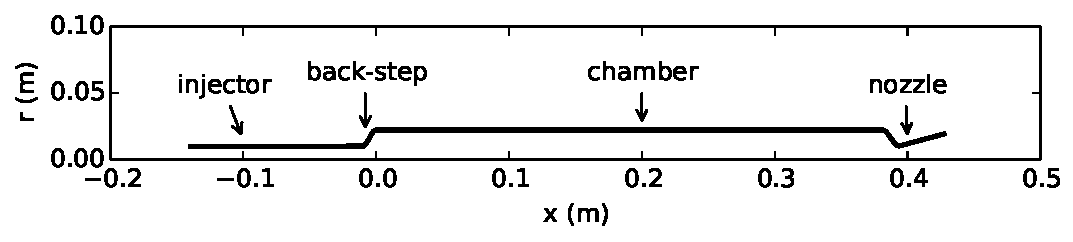
\includegraphics[width=0.8\linewidth]{pic/radius}
	\caption{Geometry of quasi-1D CVRC model.}
	\label{fig:radius}
\end{figure}

\begin{table} [h]
	\centering
	\caption{Geometry parameters of the quasi-1D CVRC with an oxidizer post length $L_{op}=14$ cm.}
	\centering
	\begin{tabular}{c c c c c c }
		\toprule
		\centering
		\multirow{2}{*}{Section} &
		\multicolumn{2}{c}{Oxidizer post} &
		\multirow{2}{*}{Chamber} &
		\multicolumn{2}{c}{Nozzle} \\
		\cmidrule(lr){2-3} \cmidrule(lr){5-6}
		& injector & back-step & & converging part & diverging part\\
		\midrule
		Length (cm) & 12.99 & 1.01 & 38.1 & 1.27 & 3.4 \\
		Radius (cm) & 1.02  & $1.02 \sim 2.25$ & 2.25 & $2.25 \sim 1.04$ & $1.04 \sim 1.95$ \\
		\bottomrule
		\label{tab:geometry_parameters}
	\end{tabular} 
\end{table}

The fuel is pure gaseous methane. The oxidizer is a mixture of 42\% oxygen and 58\% water (per unit mass). The oxidizer is injected in the oxidizer post at a temperature $T_{ox}=1030$ K so that both water and oxygen are in the gaseous phase. The operating conditions are listed in Table \ref{tab:operating-conditions}.

\begin{table} [h]
	\centering
	\caption{CVRC operating conditions.}
	\centering
	\begin{tabular}{l l l}
		\toprule
		\centering
		Parameter & Unit & Value \\
		\midrule
		Fuel mass flow rate, $\dot{m}_{f}$ & kg/s & 0.027   \\
		Fuel temperature, $T_{f}$ & K & 300   \\
		Oxidizer mass flow rate, $\dot{m}_{ox}$ & kg/s & 0.32   \\
		Oxidizer temperature, $T_{ox}$ & K & 1030   \\
		$O_2$ mass fraction in oxidizer, $Y_{O_2}$ & -- & 42.4\%   \\
		$H_2O$ mass fraction in oxidizer, $Y_{H_2O}$ & -- & 57.6\%   \\
		Mean chamber pressure & MPa & 1.34 \\
		Equivalence ratio, $E_r$ & -- & 0.8 \\
		\bottomrule
		\label{tab:operating-conditions}
	\end{tabular} 
\end{table}

For the combustion, we consider the one-step reaction model
\begin{equation*}\label{eq:combustion}
CH_4 + 2O_2 \rightarrow CO_2 + 2H_2O
\end{equation*}
We assume that the fuel reacts instantaneously to form products, allowing us to neglect intermediate species and finite reaction rates. As the equivalence ratio is less than one, there is oxidizer left after the combustion. Therefore, only two species need to be considered: oxidizer and combustion products.


The governing equations that describe the conservation of mass, momentum, and energy of the quasi-1D CVRC flow, are the quasi-1D unsteady Euler equations for multiple species, expressed in conservative form as
\begin{equation*}\label{eq:quasi-1D-equation}
\frac{\partial \mathbf{u}}{\partial t} + \frac{\partial \mathbf{f}}{\partial x} = \mathbf{s}_A + \mathbf{s}_f + \mathbf{s}_q.
\end{equation*}
The conserved variable vector $\mathbf{u}$ and the convective flux vector $\mathbf{f}$ are
\begin{equation*}\label{eq:CVRC-u-f}
\mathbf{u}= \left( \begin{gathered}
\rho A  \\
\rho uA  \\
\rho EA  \\
\rho Y_{ox} A \\
\end{gathered} \right), 
\mathbf{f} = \left( \begin{gathered}
\rho uA  \\
\left(\rho u^2 + p\right)A  \\
\left(\rho E + p\right)uA  \\
\rho uY_{ox} A \\
\end{gathered} \right),
\end{equation*}
where $\rho$ is the density, $u$ is the velocity, $p$ is the pressure, $E$ is the total energy, $Y_{ox}$ is the mass fraction of oxidizer, and $A=A(x)$ is the cross section area of the duct. The pressure $p$ can be computed using the conserved variables as
\begin{equation*}\label{eq:total-engery}
E = \frac{p}{\rho (\gamma - 1)} + \frac{u^2}{2} - C_p T_{ref},
\end{equation*}
where $T_{ref}$ is the reference temperature and is set as 298.15 K in this paper. The temperature $T$ is recovered from the equation of state $p = \rho R T$. The gas properties  $C_p$, $R$ and $\gamma$ are computed as $C_p= \sum C_{pi}Y_i$, $R=\sum R_iY_i$ and $ \gamma= C_p/(C_p-R)$, respectively. 

The source terms are
\begin{equation*}\label{eq:source-terms}
\mathbf{s}_A = \left( \begin{gathered}
0  \\
p \frac{dA}{dx}  \\
0  \\
0 \\
\end{gathered} \right), 
\mathbf{s}_f = \left( \begin{gathered}
{\dot \omega}_f  \\
{\dot \omega}_f u  \\
{\dot \omega}_f \left(h_{0}^{f} + \Delta h_{0}^{rel} \right)  \\
{\dot \omega}_{ox} \\
\end{gathered} \right), 
{\mathbf{s}_q} = \left( \begin{gathered}
0  \\
0  \\
q'  \\
0 \\
\end{gathered} \right),
\end{equation*}
where $\dot{\omega}_f$ is the depletion rate of the fuel, $\dot{\omega}_{ox}$ is the depletion rate of the oxidizer, $h_0^f$ is the total enthalpy of the fuel, $\Delta h_{0}^{rel}$ is the heat of reaction per unit mass of fuel and $q'$ is the unsteady heat release term. $\mathbf{s}_A$ accounts for area variations, $\mathbf{s}_f$ and $\mathbf{s}_q$ are related to the combustion. $\mathbf{s}_f$ represents the addition of the fuel and its combustion with the oxidizer, which in turn results in the creation of the combustion products. The depletion rate of the fuel is
\begin{equation}\label{eq:wf}
\dot{\omega}_{f}= \frac{k_f \dot{m}_f Y_{ox} \left(1+sin\xi\right)}{l_f-l_s},
\end{equation} 
where
\begin{equation*}\label{eq:xi}
\xi= -\frac{\pi}{2} + 2\pi\frac{x-l_s}{l_f-l_s}, \hspace{0.5cm} \forall \hspace{0.2cm} l_s < x < l_f.
\end{equation*}
The setting of the fuel injection restricts the combustion to the region $l_s < x < l_f$. The reaction constant $k_f$ is selected to insure that the fuel is consumed within the specified combustion zone. The depletion rate of the oxidizer is computed by 
\begin{equation*}\label{eq:wox}
\dot{\omega}_{ox} = C_{o/f} \dot{\omega}_f,
\end{equation*}
where $C_{o/f}$ is the oxidizer-to-fuel ratio.

The unsteady heat release term $q'$, also called the combustion response function, models the coupling between acoustics and combustion. In this paper, we use the combustion response function designed by Frezzotti et al. \cite{frezzotti2017numerical,frezzotti2018quasi}, which is a function of the velocity, sampled at specific abscissa $\hat{x}$ that is almost coincident with the antinode of the first longitudinal modal shape, with a certain time lag $\tau$, i.e.,
\begin{equation}\label{eq:response-function}
q'\left( x,t\right) = \alpha g\left(x\right)  A\left(x\right) \left[ u\left( \hat{x},t-\tau \right) - \bar{u}\left( \hat{x} \right) \right].
\end{equation}
Here $\bar{u}$ is the time averaged velocity, estimated with the steady-state quasi-1D model assuming $q'=0$, and $g(x)$ is a Gaussian distribution  
\begin{equation*}\label{eq:gx}
g\left(x\right)= \frac{e^{-\frac{\left(x-\mu\right)^2}{2\sigma^2}}}{\sqrt{2\pi\sigma^2}},
\end{equation*}
where $\mu$ is the mean and $\sigma$ is the standard deviation. The amount of heat release due to velocity oscillations is controlled by the parameter $\alpha$.

The boundary conditions for the quasi-1D CVRC flow include the fixed mass flow rate and the stagnation temperature at the head-end of the oxidizer injector, and the supersonic outflow at the exit of the nozzle.

Prior to unsteady simulation, the quasi-1D CVRC needs to be excited, which can be achieved by adding a perturbation to the steady-state solution. The perturbation is added by forcing the mass flow rate with a multi-sine signal
\begin{equation}\label{eq:multisine}
\dot{m}_{ox} \left(t\right)= \dot{m}_{ox,0} \left[1 + \delta\sum_{k=1}^{K}  sin\left(2\pi k\Delta f t\right) \right],
\end{equation}
where $\dot{m}_{ox,0}$ is the oxidizer mass flow rate in Table \ref{tab:operating-conditions}, $\Delta f$ is the frequency resolution and $K$ is the number of frequencies. In this paper, $\Delta f = 50 $ Hz and $K=140$, resulting in a minimal frequency of 50 Hz and a maximal frequency of 7000 Hz. $\delta$ is required to be small to control the amplitude of the perturbation and is set as 0.1\%.

The procedure of the unsteady simulation of the quasi-1D CVRC flow includes three steps:
\begin{enumerate}[(1)]
	\item  Compute the steady-state solution by setting $\dot{m}_{ox}=\dot{m}_{ox,0} $ and $q'=0$.
	\item  Excite the system by adding a perturbation to the oxidizer mass flow rate according to (\ref{eq:multisine}) and setting $q'=0$.
	\item  Perform the unsteady simulation by turning on the combustion response function $q'$ in (\ref{eq:response-function}) and turning off the oxidizer mass flow rate perturbation by setting $\dot{m}_{ox}=\dot{m}_{ox,0} $.	
\end{enumerate}


A high-fidelity quasi-1D CVRC flow solver is built by employing the MUSCL reconstruction \cite{delis1998tvd}, the Lax-Friedrichs flux \cite{shu1988efficient} and the strong stability preserving, three-stage Runge-Kutta (SSP RK3) time stepping \cite{jiang1996efficient}.

\section{Conclusions} \label{sec:con}


\bibliographystyle{plain}
\bibliography{references}

\end{document}
